\section{RADOS comme socle de Ceph} 

Après avoir défini les enjeux du stockage distribué et avoir examiné rapidement l'architecture de Ceph, nous présentons dans cette section les caractéristiques majeures de RADOS, le composant central d'un cluster Ceph.

Afin de bien comprendre la philosophie sous-jacente de RADOS, il est fondamental de bien saisir les \textbf{motivations} de la création de ce composant. Comme nous l'avons vu dans l'introduction, Ceph est né du constat que les systèmes de stockage distribués \og{}{classiques}\fg{} sont peu adaptés au stockage de volumes de données très importants, de l'ordre du petaoctet (Po) ou de l'exaoctet (Eo)\footnote{Respectivement $10^{15}$ et $10^{18}$ octets.}. 

En effet, dans le modèle traditionnel de stockage distribué, le fonctionnement entier du cluster dépend de \textbf{métadonnées}\footnote{Donnée dont l'information porte sur une autre donnée.}. Ces dernières sont fondamentales car elles permettent de localiser les données stockées sur le cluster. Leur perte ou leur altération résulte fréquemment en une impossibilité partielle ou totale d'utiliser le cluster -- une telle situation est rédhibitoire pour une entreprise. Ainsi, les métadonnées agissent comme un \textbf{SPOF}\footnote{Pour Single Point Of Failure, un point d'un système informatique dont le reste du système est dépendant et dont une panne entraîne l'arrêt complet du système.}, soit comme un risque de faille considérable pour la totalité de l'infrastructure de stockage.

Le statut sensible de ces méta-données nécessite de leur apporter un soin particulier sur le cluster, quitte les répliquer plusieurs fois. Il s'agit d'une véritable problématique, car si stocker une quantité très importante de données s'avère être un défi complexe en soi, stocker et protéger les méta-données contre les pertes éventuelles constitue un challenge supplémentaire duquel on aimerait s'affranchir. Il apparaît alors évident, à ce stade, que le modèle \og{}traditionnel\fg{} utilisant et stockant des métadonnées pour assurer le stockage distribué d'objets présente deux problèmes majeurs :

\begin{itemize}
	\item D'une part, la présence d'un SPOF est une véritable erreur de conception par rapport aux pré-requis d'un système de stockage distribué ;
    \item D'autre part, la solution consistant à répliquer toutes les méta-données est lourde et représente un véritable frein aux bonnes performances du cluster.
\end{itemize}

C'est suite à de tels constats qu'est né RADOS.

\begin{PimpedBox}
L'objectif de RADOS est, entre autres, d'assurer le bon fonctionnement d'un cluster de stockage tout en s'affranchissant des métadonnées \og{}parasites\fg{} qui rendent la montée en charge et la mise à l'échelle du cluster très difficiles.
\end{PimpedBox}

RADOS se base sur l'idée qu'un système de stockage réparti peut être soumis à un nombre important de pannes : les appareils changent d'état de disponibilité de manière continuelle. Ainsi, plutôt que de stocker des métadonnées \emph{en permanence}, les créateurs de Ceph ont eu l'idée de pouvoir les calculer \og{}\textbf{à la demande}\fg{}. Pour ce faire, RADOS repose sur un algorithme\footnote{Cet algorithme, appelé CRUSH, fait l'objet de la section \ref{chap3:sec_crush} dans laquelle il sera traité en profondeur.} qui assure la répartition pseudo-aléatoire\footnote{L'aspect pseudo-aléatoire de CRUSH signifie qu'à première vue, l'assignation d'un espace de stockage pour un objet semble être aléatoire, mais en réalité ce calcul est tout à fait déterministe et renvoie les même résultats lorsqu'il est calculé avec les même paramètres d'entrée.} des données à travers le cluster. 

L'unité de stockage utilisée par RADOS est l'\textbf{objet}. Cette approche consiste à manipuler des unités de données discrètes étiquetées par un identifiant unique. Ces objets sont gardés au sein d'un dépôt unique et stockés dans un espace d'adressage plat\footnote{Un espace de stockage plat (ou \emph{flat address space}) est un espace mémoire où chaque adresse (incrémentée de une unité en une unité, allant de 0 jusqu'à la fin de l'espace mémoire) représente une unité de donnée, \eg un objet.}, plus communément appelé \og{}\textbf{storage pool}\fg{}. Les objets ne sont pas -- comme peuvent l'être les fichiers -- imbriqués dans une succession de dossiers.
N'étant plus dans le cadre d'un système hiérarchique, les développeurs de RADOS ont dû introduire différentes \textbf{unités logiques} leur permettant de gérer la répartition d'objets distribués de façon optimale.

La suite de cette partie vise à décrire ces structures de données, dans le but d'expliquer ensuite le fonctionnement interne de RADOS.

\subsection{Les objets}

Les objets sont les plus petites unités de données dans Ceph. Ils contiennent des données à l'état binaire ainsi que les métadonnées associées, et sont étiquetées par un identifiant unique sur l'ensemble du cluster. Les objets Ceph ne sont pas restreints par une taille maximale ; ils sont stockés et répliqués sur l'ensemble du cluster. La figure \ref{chap2:objectStore} illustre la structure d'un objet.

\begin{figure}[h!]
    \centering
    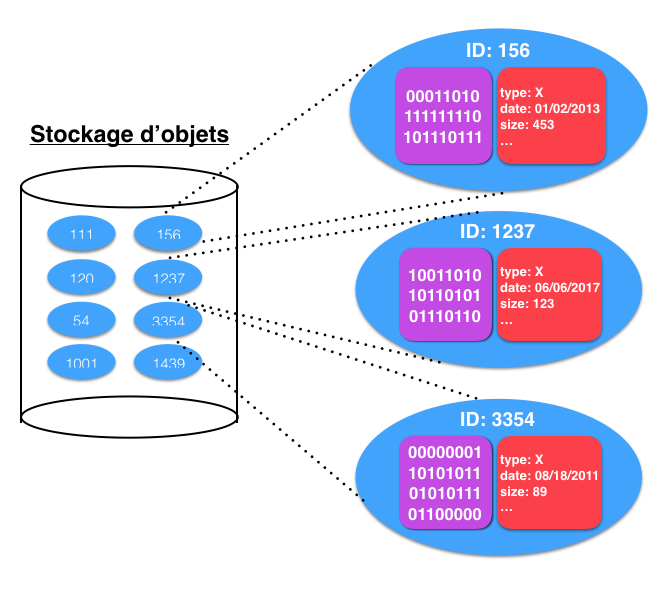
\includegraphics[width=8cm]{./images/objectStore.png}
    \caption{\label{chap2:objectStore}Aperçu du stockage d'objets.}
\end{figure}

\subsection{Les groupes de placements}

Plutôt que de manipuler chaque objet de façon indépendante, ce qui serait lourd et peu efficace, des unités logiques nommées \og{}\textbf{groupes de placements}\fg{} (en anglais, \emph{placement group} ou PG) agrègent plusieurs objets. En effet, bien que chaque objet soit identifiable par un identifiant unique, dans le cas de clusters stockant des volumes de données très importants, manipuler des millions de données indépendantes serait une tâche très coûteuse. En particulier, identifier un objet spécifique, le répliquer, et assurer une cohérence entre toutes les versions serait rédhibitoire en termes de performances. Pire encore, chaque machine ajoutée au cluster et/ou chaque nouvelle donnée stockée complexifierait davantage la manipulation d'objets.

En ce sens, il est naturel de grouper un sous-ensemble d'objets dans une structure logique ; cela permet de fortement diminuer la complexité calculatoire nécessaire à la manipulation des données. Il n'est plus question de stocker et de dupliquer un objet spécifique à chaque fois, mais plutôt de manipuler des sous ensembles d'objets\footnote{Dans la suite de ce rapport, nous utiliserons fréquemment des abus de langage en parlant de stockage ou de réplication de \emph{placement groups}. En réalité, ce sont les objets inclus dans les groupes de placement qui seront stockés et/ou répliqués. En effet, ce sont les objets qui contiennent les données du cluster. Les \emph{placement groups} sont simplement présents dans le but de réduire la complexité de l'infrastructure.}. 

\subsection{Les files}

Une file (ou \emph{pool} en anglais) est une partition logique\footnote{En d'autres termes, les pools ne concernent pas des zones mémoires contiguës, mais une vision de plus haut niveau.} dans laquelle un utilisateur de RADOS peut stocker des objets. Chaque pool contient de nombreux \emph{placement groups}, et est répliquée sur \textit{certains} nœuds du cluster. La pérennisation des données est assurée via l'utilisation de techniques de redondance telles que la réplication ou le code d'effacement (\emph{erasure coding} ou EC)\footnote{La technique d'Erasure Coding introduite dans l'une des dernières version de Ceph permet de répondre aux défauts de la technique de réplication utilisée depuis des années. En effet, dans le cas de volumes très importants de données, répliquer ces dernières augmente significativement le besoin en stockage d'un cluster. Cette technique présente donc ses limites. L'idée, ici, est de diviser les objets, d'en encoder chaque fragment, d'y ajouter des informations utiles à la restauration des données, et de stocker chacun de ces morceaux sur des machines différentes. De cette manière, en cas de mise hors service d'un/plusieurs nœud(s) du cluster, un sous ensemble des morceaux d'un objet subsistera et permettra de restaurer la totalité de l'objet. Le coût de l'\emph{erasure coding} représente 40\% du coût de la réplication. C'est une amélioration substantielle qui allège le coût de la redondance des données tout en gardant un résultat similaire à celui de la réplication}.

\subsection{Appareils de stockage d'objets}

Les appareils de stockage d'objets (\textit{Object Storage Devices} ou OSD) constituent l'un des grands concepts introduits par Ceph. Jusqu'alors, les nœuds des clusters de stockage étaient simplement destinés à stocker des données. De ce fait, toute la logique était présente dans une poignée de \textbf{nœuds maîtres} (ou \textit{master}) qui s'occupaient de gérer toute la logistique interne au cluster, et qui ordonnaient aux \textbf{nœuds esclaves} (ou \textit{slave}) d'opérer sur les données. 

Dans RADOS, en revanche, les OSD sont des appareils de stockage tirant profit de leur \textbf{intelligence} inhérente ; ils sont une composante à part entière de la logique du système reparti. Leur structure est la suivante: 

\begin{itemize}
	\item Un processeur (CPU) ;
	\item De la mémoire vive (RAM) ;
    \item Une interface réseau ;
    \item Un espace de stockage (disque dur ou RAID\footnote{La technologie RAID (Redundant Array of Independent Disks), ou \og{}Ensemble redondant de disques indépendants\fg{}, consiste à mettre en grappe plusieurs disques durs pour en obtenir une partition logique unique. Ainsi, à partir de plusieurs disques durs physiques, on obtient un seul espace visible par le système d’exploitation. En fonction de l’objectif, le RAID permet d'accroître la performance d’accès et d’écriture des données ou d'améliorer la sécurité des informations.}).
\end{itemize}

Pour assurer le fonctionnement du cluster, ces derniers communiquent à l'aide de protocoles de type pair-à-pair\footnote{La particularité des architectures pair-à-pair réside dans le fait que les données puissent être transférées directement entre deux postes connectés au réseau, sans transiter par un serveur central. (source : \url{https://fr.wikipedia.org/wiki/Pair\_à\_pair})}. 

\begin{PimpedBox}
Dans le but de conserver des performances optimales, RADOS se base sur un ensemble de structures logiques facilitant la manipulation de grandes quantités d'objets distribués à travers le cluster. Ces structures interagissent entre elles pour garantir la cohérence des données dupliquées et la reprise après erreur lorsqu'un problème survient sur le cluster. 
\end{PimpedBox}

L'étude des mécanismes internes à RADOS est abordée dans la suite de cette partie.

\subsection{Gestion de la répartition des objets}

Afin de gérer la répartition des données dans le cluster, RADOS utilise un \textbf{algorithme de placement} nommé \textbf{CRUSH}\footnote{CRUSH signifie Controlled Replication Under Scalable Hashing, littéralement \og{}Réplication contrôlée par hachage extensible\fg{}. Les objectifs de cet algorithme sont brièvement présentés dans cette partie. La partie \ref{chap3:sec_crush} est dédiée à l'étude approfondie de ses caractéristiques.}. Cet algorithme permet, à partir d'un identifiant d'objet ou d'un groupe de placement, de \textbf{calculer} la liste des OSD responsables de leur stockage. En ce sens, l'algorithme CRUSH permet de déterminer des métadonnées \og{}à la demande\fg{}, permettant d'assigner\footnote{L'assignation de groupes de placements aux OSD se fait \textit{pseudo-aléatoirement}. En d'autres termes, l'observation extérieure des résultats de l'algorithme semble indiquer que la répartition des données est totalement aléatoire dans le cluster. En revanche, CRUSH est un algorithme déterministe, et s'assure de répartir la charge de travail équitablement sur l'ensemble des nœuds du cluster.} des groupes d'objets à des OSD tout en repartissant la charge de stockage de façon uniforme sur l'ensemble du cluster.

\subsubsection{Gestion interne du cluster et cohérence des données}

Alors que CRUSH permet de calculer la position des données dans l'infrastructure de stockage, ce sont les OSD, qui, ensuite, assurent le \textbf{fonctionnement} du cluster. En effet, dans un cluster de milliers de machines, les pannes et les reprises après erreurs peuvent être très fréquentes. De ce fait, l'état du cluster est amené à changer très régulièrement. Pour en faciliter la gestion, cet état est entièrement représenté par une \textbf{carte}, la \emph{cluster map}\footnote{En réalité, cette \emph{cluster map} est un conglomérat de \og{}cartes\fg{} différentes. Elle englobe la carte des OSD, la carte des groupes de placement, la carte de CRUSH, la carte des moniteurs, et, enfin, la carte des serveurs de métadonnées.}, faisant l'inventaire de tous les OSD étant dans le cluster.

Plutôt que de n'être présente que sur un nœud spécifique -- ce qui introduirait un point de faille unique dans l'infrastructure --, cette structure est dupliquée sur tous les nœuds du cluster, ainsi que sur les clients qui interagissent avec RADOS. Il serait impensable, en revanche, de devoir mettre à jour la carte du cluster sur l’ensemble des nœuds chaque fois qu'un OSD devient indisponible ou est ajouté. L'opération serait bien trop coûteuse et diminuerait significativement les performances globales, agissant comme un \textit{goulot d'étranglement}. 

Pour adresser cette problématique, la carte est \textbf{datée} par une époque\footnote{Notons que l'utilisation d'une époque (\emph{epoch} en anglais) pour gérer les versions de la carte du cluster fait écho aux horloges de Lamport (estampilles) que nous avons étudié en SR05.} représentant sa version\footnote{Plus la valeur de l'époque est petite, plus la carte du cluster est ancienne.}. Ajouter l'époque de la carte détenue par chaque OSD aux messages qu'il émet permet aux autres nœuds du cluster de se mettre d'accord sur la distribution des données à l'instant de leur communication. En d'autres termes, l'échange de leur version de la carte leur permet de savoir si leur information est à jour, ou si elle nécessite d'être enrichie. De cette manière, les  changements d'état du cluster peuvent être transmis de proche en proche à mesure que les OSD communiquent. Cette méthode de mise à jour des nœuds du cluster, appelée \textbf{lazy update}\footnote{Littéralement \og{}mise à jour fainéante\fg{}, faisant référence à l'absence de mise à jour systématique, comme dans l'algorithme de \textit{snapshot} avec lestage.}, permet de ne pas surcharger le réseau interne à l'infrastructure. Les mises à jour sont propagées de proche en proche en cas de besoin.

En revanche, pour garder un état global cohérent, ces actualisations doivent tout de même circuler relativement rapidement d'un OSD à un autre. Pour ce faire, les OSD émettent des messages dits \og{}\textbf{heartbeat}\fg{}, ayant la double particularité pour un nœud de savoir si ses voisins sont toujours en train de s’exécuter\footnote{\ie l'OSD voisin n'est pas devenu indisponible suite à une erreur.}, et de recevoir la version de la carte du cluster de ses voisins de façon fréquente et régulière. Avec cette technique, les OSD peuvent fréquemment demander les mises à jour incrémentales\footnote{Lorsque deux cartes de cluster (c1 et c2 avec $c1.epoque > c2.epoque$) n'ont pas la même version, cela signifie que l'une est plus récente que l'autre. De cette manière, le nœud ayant l'époque la plus faible peut demander à son voisin de le mettre à jour, et de l'informer des changements qu'a subit l’infrastructure durant la période de temps $c1.epoque - c2.epoque$. Cette mise à jour est faite en envoyant une succession de messages dont chacun décrit un événement ayant eu lieu sur l’infrastructure, et ce jusqu’à ce que l'OSD le moins à jour ait une époque égale à $c1$. De cette manière, chaque OSD est assuré d'avoir en sa connaissance chaque événement étant arrivé sur le cluster. L'historique est connu de tous les nœuds du cluster et chaque distribution intermédiaire de donnée est prise en compte. Cette technique élégante donne les moyens à chaque OSD de mettre à jour ses voisins, et la cohérence des données est assurée.} nécessaires à leur remise à jour. 

Enfin, en cas de non-réception répétée des messages de \emph{heartbeat} d'un voisin, un OSD peut prendre la décision de notifier le problème à un nœud dit \textbf{moniteur}. Ces nœuds n'ayant jusqu'alors pas été mentionnés ont pour rôle général de \textbf{conserver la version maître} de la carte du cluster. Pour ce faire, ils \textbf{votent} un consensus permettant de conserver une version \textbf{stable} et la plus \textbf{à jour} possible de la carte maître. En particulier, l'état d'un nœud soupçonné \og{}hors service\fg{} sera mis à jour par leurs soins, et l'OSD sera répertorié comme étant \emph{down}\footnote{À savoir que l'état d'un OSD est défini par un couple dont le premier membre indique si l'appareil est joignable (\emph{up}) ou pas (\emph{down}), et dont le second membre renseigne sur l'inclusion du nœud dans la carte du cluster (\emph{in} ou \emph{out}).}, avant que les placement groups qu'il stockait soient confiés à d'autres OSD du cluster.

\subsubsection{\og{}CRUSH lookup\fg{} et interactions avec les utilisateurs}

Lorsqu'un utilisateur souhaite interagir avec RADOS, ce dernier doit se munir d'une carte du cluster pour avoir une idée de la répartition des données et avoir connaissance des OSD qui constituent l'infrastructure. Pour ce faire, l'utilisateur initie l'échange avec les nœuds \textbf{moniteurs}\footnote{Pour les interactions suivantes, l'utilisateur pourra directement communiquer avec les OSD. Sa copie locale de la \emph{cluster map} recevra les modifications incrémentales nécessaires à sa remise à jour si son époque est trop faible. Cela évite au cluster de devoir mettre les clients à jour à mesure que l'état interne évolue.} pour obtenir une carte du cluster. Il pourra alors stocker des objets dans une \emph{pool} et utiliser l'algorithme CRUSH pour déterminer l'emplacement de stockage de la donnée. Cette étape se nomme \textbf{CRUSH lookup}, et nécessite la détention de la carte du cluster. 

L'emplacement déterminé par le CRUSH lookup est égal à l'identifiant de l'OSD sur lequel sera faite la demande en écriture de l'objet à stocker. Cet OSD est dit \textbf{primaire} (ou \emph{Primary OSD})\footnote{Un OSD primaire est responsable, pour un placement group au sein du cluster, de s'assurer que les données du PG restent cohérentes. Notons qu'un OSD peut être primaire pour un placement group, et secondaire pour un autre ; c'est d'ailleurs ce qu'il se passe en pratique} pour le placement group. Son rôle est de prendre en charge la gestion de la répartition du placement group au sein du cluster. 

Le processus de stockage d'un objet par un utilisateur peut être résumé par la séquence suivante :

\begin{enumerate}
	\item L'objet est placé dans un placement group ;
    \item Le placement group est placé dans une file ;
    \item Le mécanisme de CRUSH lookup calcule l'identifiant de l'OSD primaire sur lequel écrire le PG ;
    \item L'OSD en question, une fois la demande reçue, utilise la version de la carte du cluster qu'il détient pour répliquer le placement group $n$ fois\footnote{Les conditions de réplications des placements group sont configurées dans la \emph{pool}.}.
    \item L'OSD primaire renvoie un message d'\textbf{acquittement} (\og{}ACK\fg{}) à l'utilisateur après avoir reçu \textbf{tous} les acquittements des OSD \textit{secondaires}\footnote{Les OSD secondaires sont ceux contenant les réplicas du placement group.}. Cet ACK est caractéristique d'une réplication réussie\footnote{On notera là encore, un parallèle fort avec les notions de vagues et d'ondes vues en cours de SR05, et plus particulièrement avec l'algorithme de calcul diffus.}.
\end{enumerate}

De cette manière, le coût lié à la réplication des données est déporté au sein du réseau interne à l'infrastructure lors de sa prise en charge par les OSD du cluster. Cet ensemble d'OSD (primaire et secondaires) forme ce qui est plus communément appelé un \textbf{acting set}\footnote{Liste ordonnée d'OSD responsables du stockage d'un placement group.}. L'OSD primaire est donc responsable, pour un placement group, du processus de \textbf{peering}, qui vise à assurer l’intégrité des informations parmi les différents OSD de l'acting set d'un placement group. 

\begin{PimpedBox}
C'est l'OSD primaire -- dont l'identifiant est calculé lors du CRUSH lookup effectué par l'utilisateur -- qui sera en mesure d'accepter la première requête d'écriture venant du client, et qui assurera le processus de la réplication et d'acquittement à l'utilisateur.
\end{PimpedBox} 

\subsubsection{Reprise après erreurs et élections des OSD primaires}

Chaque OSD sait lorsqu'il est secondaire pour un groupe de placement donné. De ce fait, en cas d'indisponibilité de l'OSD primaire, suite à une erreur quelconque, c'est l'OSD secondaire suivant immédiatement l'OSD primaire dans l'acting set qui est élu OSD primaire. Pour garantir la cohérence des données après une élection, les OSD secondaires envoient tous des messages de \textbf{notification} (ou \emph{Notify}) à l'OSD primaire afin que ce dernier découvre son rôle d'\og{}élu\fg{}\footnote{L'envoi de messages de notifications des OSD secondaires vers le nouvel OSD primaire permet d'éviter à ce dernier de devoir considérer l'ensemble des placements groups qu'il stocke pour trouver celui pour lequel il est devenu primaire.}, et puisse enclencher le processus de \textbf{peering}\footnote{Le processus de peering consiste à faire en sorte que tous les OSD d'un acting set soient en accord à propos de l'état des objets inclus dans un placement group donné. Notons qu'être en accord sur l'état du placement group ne signifie en rien que tous les OSD doivent tous avoir la version la plus récente du PG.}. 

Pour assurer son rôle d'OSD primaire, le site élu contacte tous les OSD ayant fait partie de l'acting set du placement group pour lequel il est devenu responsable, dans le but de rassembler toutes les données et métadonnées associées. De cette manière, l'OSD primaire construit un historique des modifications apportées sur le placement group, et est alors en mesure de connaître la version la plus récente que chaque réplicat devrait avoir. Le site élu obtient également l'historique de tous les journaux concernant le placement group. 

A l'aide de ces journaux, l'OSD primaire sait ce à quoi devrait \og{}ressembler\fg{} le placement group sur chaque site secondaires. De ce fait, il peut, en cas de reprise après erreur d'un site de l'acting set, lui envoyer l'information nécessaire à sa reprise. 

\begin{PimpedBox}
L'OSD primaire prend en charge la gestion de la reprise après erreur concernant les données pour lesquelles il est responsable. Il peut informer chacun de ses sites secondaires de l'état que devrait avoir leur réplicas, de sorte à ce que ces derniers amorcent la démarche de reprise en arrière-plan.
\end{PimpedBox}

De ce fait, en cas d'interruption de l'OSD primaire, c'est l'OSD secondaire qui lui succède par défaut, et, les autres OSD de l'acting set lui notifient son changement de statut. Suite a cela, le nouvel OSD primaire rassemble toutes les données lui permettant d'avoir une vue d'ensemble sur l'état de chaque répliquas du placement group. De cette manière, le site élu est en mesure de coordonner la reprise après erreur concernant le placement group pour lequel il est responsable.

\subsection{Les moniteurs}

\begin{PimpedBox}
Le rôle principal des moniteurs Ceph consiste à conserver une copie maître de la carte du cluster. Ils fournissent également des services d'authentification et de journalisation.
\end{PimpedBox}

Avant qu'un client Ceph puisse accéder en lecture ou écriture aux données du cluster, celui-ci doit contacter un moniteur afin d'obtenir la plus récente copie de la carte du cluster. Suite à cela, le client peut calculer l'emplacement de n'importe quel objet sur le cluster.

Un cluster de stockage Ceph peut fonctionner avec un seul moniteur. En revanche, un tel cas de figure introduit un point de faille unique. De ce fait, il est recommandé, pour tolérer les pannes, et assurer une fiabilité maximale, de configurer un ensemble impair\footnote{Quorum et split-brain.} de nœuds moniteurs. 

Nous détaillons le fonctionnement interne des moniteurs -- en particulier dans leur mécanisme de \textbf{consensus} -- dans la section \ref{chap2:sec3}

\section{Consensus des moniteurs}
\label{chap2:sec3}

Cette section se propose d'expliquer le fonctionnement du consensus des moniteurs. En effet, dans le cas d'un groupe de moniteur, les actions de décision doivent être cohérentes. Comme l'utilisation de plusieurs moniteurs est quasi obligatoire pour garantir l'absence de SPOF, il est important d'en comprendre le fonctionnement.

\subsection{Paxos, une solution pour surveiller l'état du cluster}

Une des difficultés principales intrinsèques aux systèmes distribués est l'obtention d'une certaine fiabilité dans des décisions distribuées. Il s'agit du problème largement étudié du \textbf{consensus}. Dans notre cas, les moniteurs cherchent en permanence à se mettre d'accord sur l'\textbf{état} du cluster.

Pour traiter ce problème, les moniteurs Ceph utilisent un algorithme de type \textbf{Paxos}, une famille de protocoles permettant de résoudre ce problème du consentement. Ces algorithmes sont connus pour être complexes ; nous en proposons une explication.

\subsection{Comment fonctionne Paxos ?}

Un nœud Paxos peut prendre l'un des trois rôles suivants, de manière non-exclusive : \textbf{proposant} \textit{ou} leader, \textbf{accepteur} et \textbf{apprenant} :

\begin{itemize}
\item Un proposant (pas nécessairement unique) propose une valeur sur laquelle il souhaite un accord. Pour ce faire, il envoie une proposition contenant une valeur à l'ensemble de tous les accepteurs, qui décident d'accepter ou non la valeur.
\item Chaque accepteur choisit une valeur de manière indépendante -- il peut recevoir plusieurs propositions, chacune d'un autre proposant -- et envoie sa décision aux apprenants, qui déterminent si une valeur a été acceptée.
\item Une fois que la majorité des nœuds ont accepté, un consensus est atteint et le coordinateur diffuse un message de validation à tous les nœuds.
\end{itemize}

En pratique, un seul nœud peut prendre plusieurs ou tous ces rôles, mais dans les exemples de cette section, chaque rôle est exécuté sur un nœud distinct, comme illustré figure \ref{chap2:paxos_arch}.

\begin{figure}[H]
    \centering
    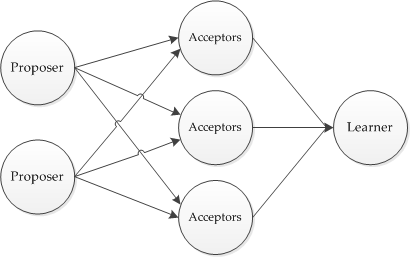
\includegraphics[width=9cm]{./images/paxos_basic_archi.png}
    \caption{\label{chap2:paxos_arch}Architecture basique de Paxos}
\end{figure}

\subsection{Étude de Paxos à travers un exemple}

Dans l'algorithme Paxos standard, les proposants envoient deux types de messages aux accepteurs : \og{}prépare\fg{} et \og{}accepte\fg{} les demandes. Dans la première étape de cet algorithme, un proposant envoie une demande de préparation à chaque accepteur contenant une valeur proposée ($v$) et un numéro de proposition ($n$). 

Le numéro de proposition de chaque proposant doit être un entier naturel, monotone et unique au regard des numéros de propositions d'autres proposants.

Dans l'exemple illustré figure \ref{chap2:paxos_ex1}, il y a deux proposants, tous deux faisant des demandes de préparation. La demande du proposant A atteint les accepteurs X et Y avant la demande du proposant B, mais la demande du proposant B atteint l'accepteur Z d'abord.

\begin{figure}[H]
    \centering
    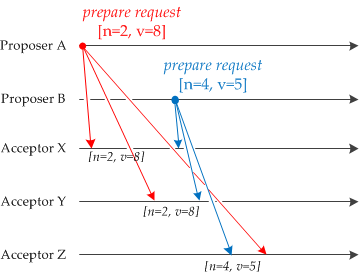
\includegraphics[width=8cm]{./images/paxos_ex1.png}
    \caption{Phase de préparation : prepare request.}
    \label{chap2:paxos_ex1}
\end{figure}

Si l'accepteur recevant une demande de préparation n'a pas vu une autre proposition, l'accepteur répond avec une réponse préparatoire qui promet de ne jamais accepter une autre proposition avec un nombre de propositions inférieur. Ceci est illustré dans la figure \ref{chap2:paxos_ex2}, qui montre les réponses de chaque accepteur à la première demande de préparation qu'ils reçoivent.

\begin{figure}[H]
    \centering
    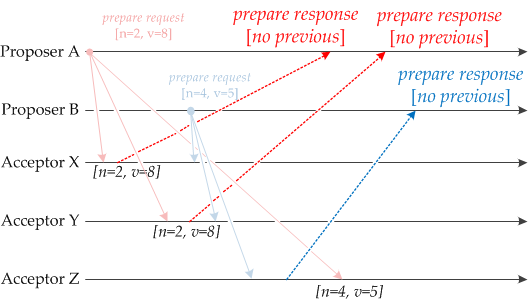
\includegraphics[width=8cm]{./images/paxos_ex2.png}
    \caption{Phase d'acceptation n°1: prepare response.}
    \label{chap2:paxos_ex2}
\end{figure}

Finalement, l'accepteur Z reçoit la demande du proposant A et les accepteurs X et Y reçoivent la demande du proposant B. Si l'accepteur a déjà vu une demande avec un numéro de proposition plus élevé, la demande de préparation est ignorée, comme c'est le cas avec la demande du proposant A à l'accepteur Z. Si l'accepteur n'a pas vu une demande numérotée plus élevée, il promet encore d'ignorer toute demande avec des numéros de proposition inférieurs, et renvoie la proposition la plus élevée qu'elle a acceptée avec la valeur de cette proposition. C'est le cas avec la demande du proposant B aux accepteurs X et Y, comme illustré figure \ref{chap2:paxos_ex3}.

\begin{figure}[H]
    \centering
    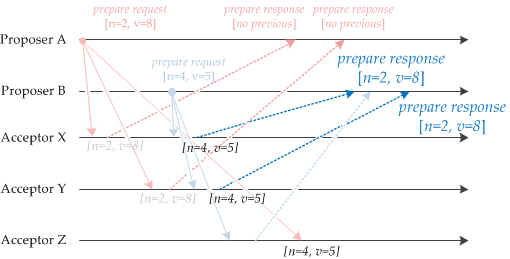
\includegraphics[width=8cm]{./images/paxos_ex3.png}
    \caption{Phase d'acceptation n°2: prepare response.}
    \label{chap2:paxos_ex3}
\end{figure}

Une fois que le proposant a reçu la préparation des réponses d'une majorité d'accepteurs, il peut émettre une demande d'acceptation. Étant donné que le proposant A n'a reçu que des réponses indiquant qu'il n'y avait pas de propositions précédentes, il envoie une demande d'acceptation à chaque accepteur avec le même numéro de proposition et la même valeur que sa proposition initiale (n = 2, v = 8). Cependant, ces demandes sont ignorées par tous les accepteurs, car toutes ont promis de ne pas accepter les demandes avec un numéro de proposition inférieur à 4 (en réponse à la demande de préparation du proposant B).

Le proposant B envoie une demande d'acceptation à chaque accepteur contenant le numéro de proposition qu'il a utilisé précédemment (n = 4) et la valeur associée au numéro de proposition le plus élevé parmi les messages de préparation de réponse reçus (v = 8). Notons que ce n'est pas la valeur proposée initialement par le proposant B, mais la valeur la plus élevée des messages de préparation de réponse qu'il a vu. Cette phase de confirmation est illustrée figure \ref{chap2:paxos_ex4}.

\begin{figure}[H]
    \centering
    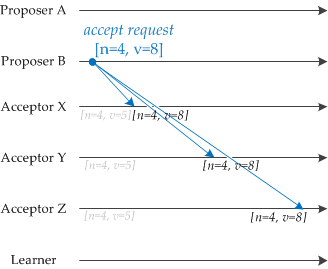
\includegraphics[width=8cm]{./images/paxos_ex4.png}
    \caption{Phase de confirmation : accept response.}
    \label{chap2:paxos_ex4}
\end{figure}

Enfin, si un accepteur reçoit une demande d'acceptation pour un numéro de proposition supérieur ou égal à celui déjà vu, il accepte et envoie une notification à chaque nœud de l'apprenant. Une valeur est choisie par l'algorithme de Paxos lorsqu'un apprenant découvre qu'une majorité d'accepteurs ont accepté une valeur. Cette dernière phase est illustrée figure \ref{chap2:paxos_ex5}.

\begin{figure}[H]
    \centering
    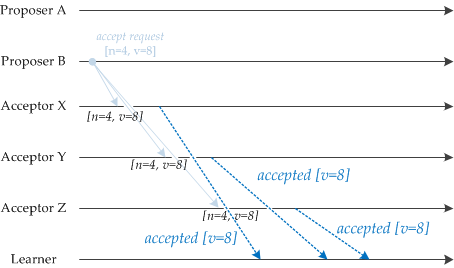
\includegraphics[width=8cm]{./images/paxos_ex5.png}
    \caption{Consensus atteint : accepted.}
    \label{chap2:paxos_ex5}
\end{figure}

Une fois qu'une valeur a été choisie par Paxos, une communication ultérieure avec d'autres proposants ne peut pas modifier cette valeur. Si un autre proposant (C) envoie une demande de préparation avec un numéro de proposition supérieur à celui déjà vu, et une valeur différente (par exemple, n = 6, v = 7), chaque accepteur répond avec la proposition la plus élevée précédente (n = 4, v = 8). Cela requiert l'auteur C d'envoyer une demande d'acceptation contenant [n = 6, v = 8], ce qui confirme la valeur qui a déjà été choisie. En outre, si une minorité d'accepteurs n'a pas encore choisi de valeur, ce processus garantit qu'ils atteignent éventuellement un consensus sur la même valeur.

\subsection{Intégration de Paxos dans Ceph}

La figure \ref{chap2:paxos_ceph} illustre l'intégration et la place de Paxos dans Ceph.

\begin{figure}[H]
    \centering
    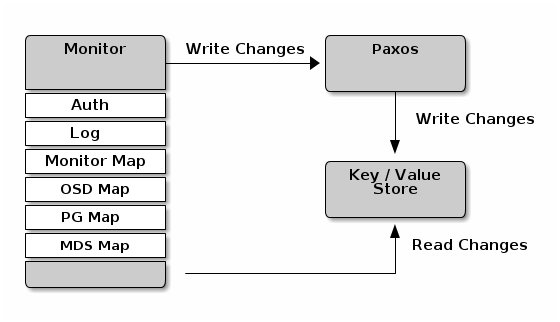
\includegraphics[width=8cm]{./images/ceph_paxos.png}
    \caption{Application de Paxos dans Ceph}
    \label{chap2:paxos_ceph}
\end{figure}

Les moniteurs écrivent toutes les modifications de la carte du cluster dans une instance Paxos, qui va elle-même écrire ces modifications dans un magasin de clés/valeurs. Ces modifications sont ensuite exploitées par les autres moniteurs Ceph afin de mettre leur version de la carte du cluster à jour lors d'opérations de synchronisation.